\chapter{Results}
\label{chap5}
\textit{This chapter presents the results of the experiments and evaluations conducted in this research. It provides a detailed analysis of the performance of MBRL algorithms with continuous training and provide insights into the research questions posed at the beginning of this study.}

\section{Surrogate Model Performance}
\subsection{Performance Evaluation}
To evaluate the surrogate model's performance, it is important to consider several critical metrics. These metrics serve as crucial indicators of how effectively the model approximates and forecasts the robot's behavior. Here, these metrics are elaborated without delving into details:
\begin{itemize}
    \item Average Steps before Failure: This metric assesses the model's capacity to predict the duration of a simulation run without encountering failure, serving as an indicator of sample efficiency.
    \item Validation RMSE and Validation Loss: This RMSE quantifies the disparity between the surrogate model's predictions and the actual values present in the validation dataset, as defined in Equation \ref{eq:RMSE}. Lower RMSE values are indicative of a higher degree of precision and accuracy in forecasting future states ($s_{t+1}$). Concurrently, the Validation Loss serves as an overarching measure of the model's performance on the validation dataset, underscoring the significance of minimizing this metric to enhance predictive capabilities, as defined in Equation \ref{eq:loss}.
    \item NRMSE: NRMSE provides a normalized measure of error, enabling comparisons of prediction accuracy across expert pattern datasets. It proves particularly valuable in evaluating the surrogate model's ability to predict sensor observations on the robot. The single step prediction NRMSE is calculated by Equation \ref{eq:NRMSE}, the long-term prediction NRMSE is calculated by Equation \ref{eq:NRMSET}.
    \item Correlation Coefficient ($R$): The $R$ quantifies the linear relationship between simulated and predicted values, as specified in Equation \ref{eq:R}. A higher $R$ signifies a more robust correlation, highlighting the model's proficiency in capturing underlying data trends and patterns.
\end{itemize}

\subsection{Control Variables Restriction}
The investigation commences with a focused exploration of state-space restriction within the surrogate model. The state-space, encompassing both observations and actions, is defined as $\mathbf{s}_t = [\pmb{\theta}(t), \mathbf{v}(t), \mathbf{f}n(t), \mathbf{a}_{t-1}]$ in Section \ref{sec:ss}. It is worth noting that the first three terms in this state-space originate from observations and are inherently challenging to restrict, but the action space can be subject to constraints.  It's crucial to acknowledge that the first three terms in this state-space comes from observations and present inherent challenges for restriction, but the action space can indeed be subjected to constraints. 

An important aspect to underscore is that the restriction of the robot's action space was achieved through the application of pattern-defined modeling techniques. Specifically, the robot's legs are interconnected in diagonal pairs, similar to a trotting pattern. This inherent structural arrangement significantly simplifies the action space compared to dealing with the complexity of controlling 12 individual motor actions\cite{jiSynthesizingOptimalGait2022}, effectively reducing it from $\mathbf{a}\in\mathbb{R}^{12}$ to $\mathbf{a}\in\mathbb{R}^4$. 

Furthermore, an alternate method of parameterization was applied, where the surrogate model's configuration incorporates specific control variables. Within this context, the actions are as defined in Section \ref{Sec:as}, taking the form of $\mathbf{a}_{t} = [\alpha_{b_1}, z_{l_1},\alpha_{b_2},z_{l_2}]$. These variables are subject to the bounds governed by the gains ($\alpha_{b_{gain}}\, , z_{l_{gain}}$). It's also crucial to emphasize that these gains associated with actions hold significance not only in the construction of the surrogate model but also play a vital role in shaping the behavior and adaptability of the SoftQ. Therefore, our focus centers on two key components within the action space: the gain of bending angle $\alpha_{b_{gain}}$ and the gain of compression length $z_{l_{gain}}$ for each of the diagonal leg pairs. To address this aspect, a series of simulations involving random actions within a bounded action space were carried out. These simulations aimed to gather the necessary data required for training the surrogate model. Subsequently, the performance of the trained model was evaluated. To effectively assess the trained neural networks performance, a color heat map can be employed to provide a visual representation of various performance metrics, as shown in Figure \ref{fig:NN_heat}. Each metric is associated with a specific color scale, allowing for a quick and intuitive evaluation.

\begin{figure}[htb]
    \centering
    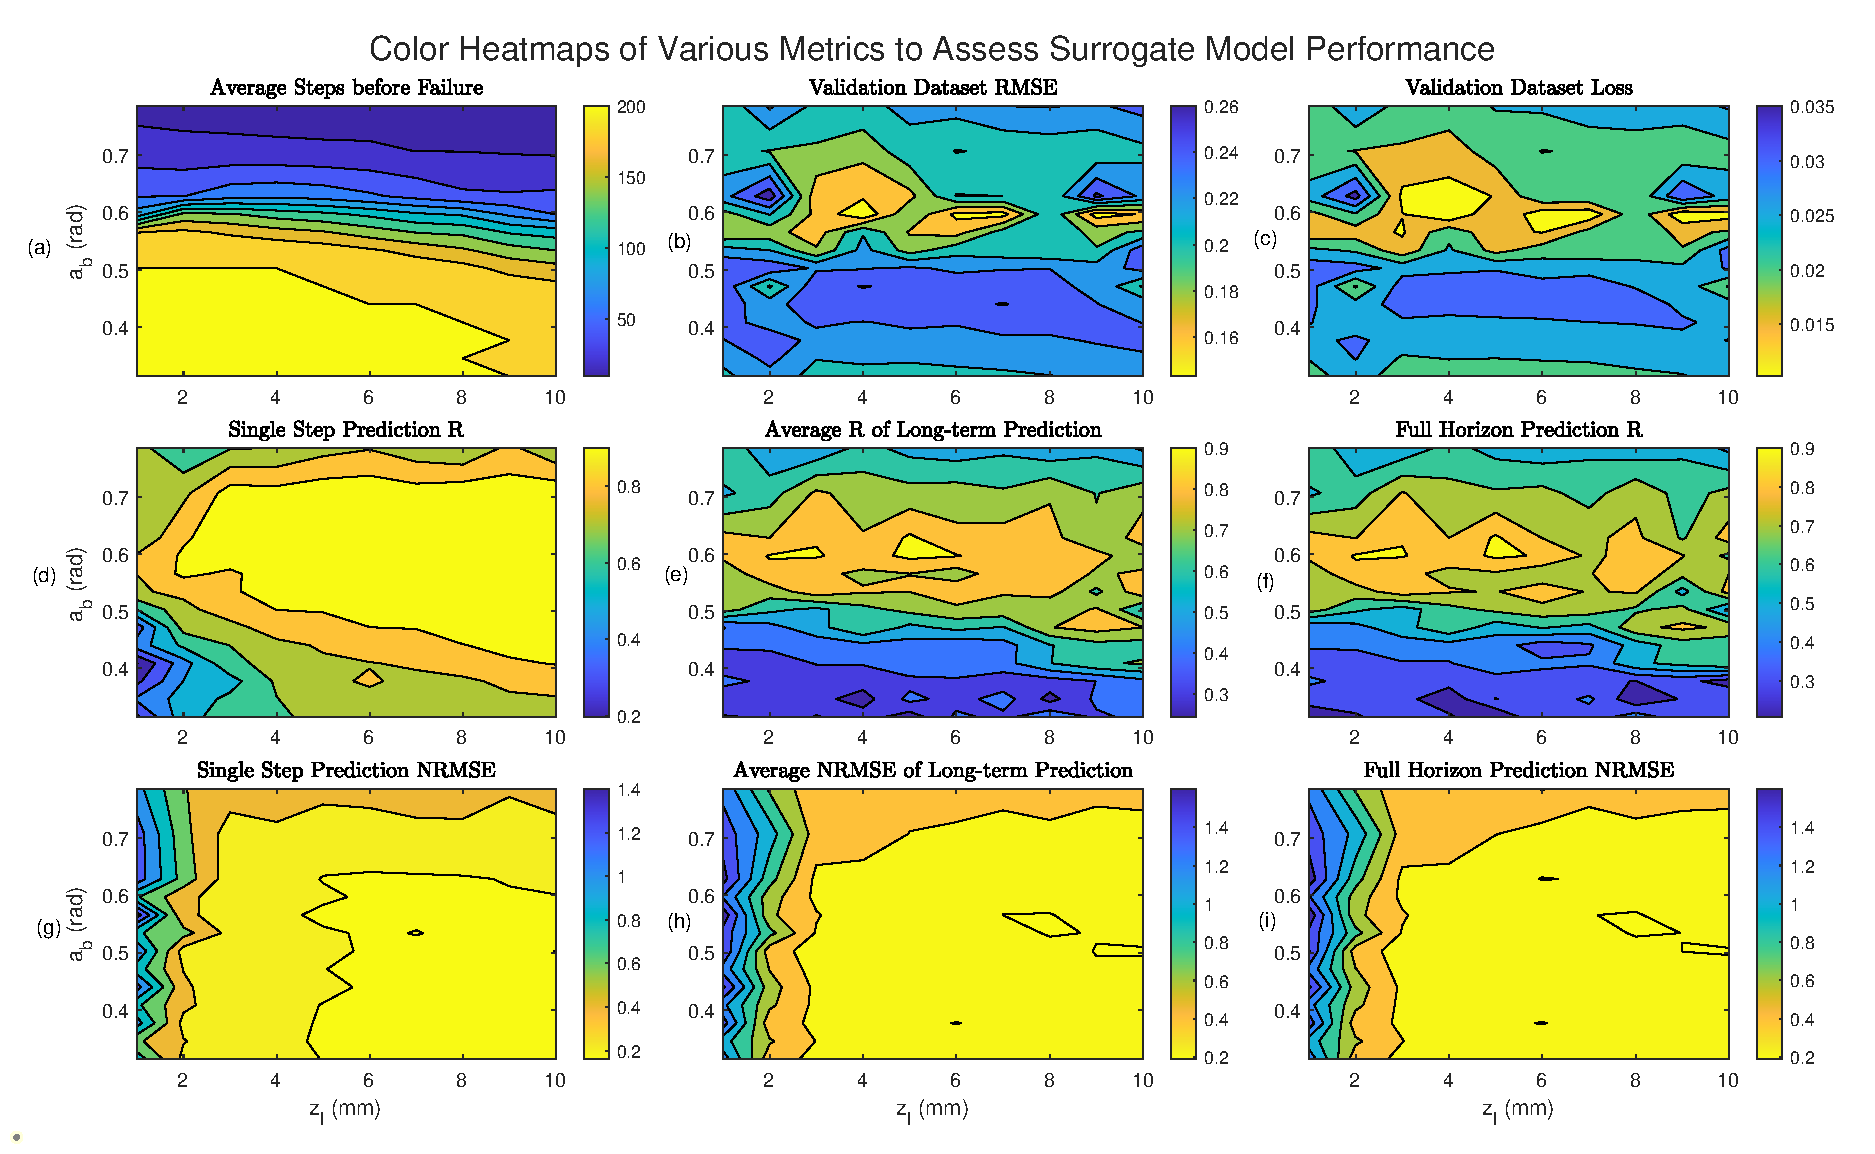
\includegraphics[width=\linewidth]{img/chap5/NN_heat.eps}
    \caption{Visualization of Performance Metrics Through Color Heat Map for Evaluating Trained Surrogate Models. The metrics include: (a) Average Steps before Failure; (b) \ac{RMSE} on the Validation Dataset; (c) Loss on the Validation Dataset; (d) Single Step Prediction Coefficient R; (e) Average Coefficient $R$ for Long-term Prediction; (f) Coefficient $R$ for Full Horizon Prediction; (g) NRMSE for Single Step Prediction; (h) Average NRMSE for Long-term Prediction; (i) NRMSE for Full Horizon Prediction.}
    \label{fig:NN_heat}
\end{figure}

In Figure \ref{fig:NN_heat}(a), it is evident that reducing the lower restrictions within the action space leads to an increase in the average number of steps the system can take before encountering failure, indicating improved data efficiency due to reduced locomotion risk with smaller actions. In Figure \ref{fig:NN_heat}(c), all neural networks converge with a loss below 0.037 in the validation dataset, with minimal differences between them. In Figure \ref{fig:NN_heat}(b), validated in the same dataset, RMSE converges to a minimum level. Notably, better validation RMSE is achieved when $\alpha_b$ ranges from 0.55 to 0.7 radians and $z_l$ ranges from 3 to 9 millimeters, suggesting optimal model performance within these parameter ranges.

In assessing single-step predictions using various expert gait pattern datasets, the correlation coefficient ($R$) between predictions and ground truth was calculated, as depicted in Figure \ref{fig:NN_heat}(d). The results show consistently high accuracy when either the compression length ($z_l$) or the bending angle ($\alpha_b$) is high, or when both are elevated. This observation aligns with the expectation that for the robot to achieve higher speeds, it should exhibit more pronounced behaviors, which are characterized by larger values of these parameters. Consequently, the expert gait dataset used in this context emphasizes high values of $\alpha_b$ and $z_l$, resulting in smaller differences between predictions and ground truth, and consequently, lower values of R. A similar trend is observed when considering single-step predictions. Smaller NRMSE values are associated with high values of $z_l$ and $\alpha_b$, but interestingly, low $\alpha_b$ values also yield small NRMSE values. This implys that bending angle ($\alpha_b$) exerts a more significant influence on robot locomotion. These results are visually represented in Figure \ref{fig:NN_heat}(g). However, it is important to note that neither the NRMSE nor $R$ reach their lowest points in the highest $\alpha_b$ region, suggesting poorer predictions when too small steps are taken before simulation failure, resulting in an insufficient amount of useful data.

For multi-step predictions on the same expert gait pattern datasets, the effects of $\alpha_b$ and $z_l$ are similar in single step prediction, but the models with low $\alpha_b$ values perform less effectively in predicting over longer time horizons, suggesting a lack of robust generality in these models. However, as shown in Figure \ref{fig:NN_heat}(e), the average correlation coefficient ($R$) for long-term predictions reveals that models with relatively high values of both $\alpha_b$ and $z_l$ struggle to predict states over extended horizons. This challenge could be attributed to the larger action space, which introduces more unpredictability and subsequently leads to reduced performance compared to models with lower $z_l$ values when trained on the same dataset size. This trend is also evident in the full horizon prediction R, as depicted in Figure \ref{fig:NN_heat}(f), where predictions at relatively high values of both $\alpha_b$ and $z_l$ deteriorate. In addition, the average NRMSE of long-term predictions exhibits a similar performance to what was observed in single-step predictions, which shows different patterns compared to $R$ results, because the NMRMSE is normalised and large values like contact forces may have more effects on the metrics. Lower errors are associated with larger values of $\alpha_b$ and $z_l$, but NRMSE also decreases when $\alpha_b$ reaches its highest values. These results are presented in Figure \ref{fig:NN_heat}(h). Interestingly, performance remains consistent when $\alpha_b$ is smaller than 0.72 radians and $z_l$ is larger than 3 millimeters. Likewise, in the case of NRMSE for full horizon prediction, there is no significant change in performance, as indicated in Figure \ref{fig:NN_heat}(i).

Hence, the optimal action state restrictions can be identified as approximately $\alpha_b$ around 0.6 rad and $z_l$ around 7 mm. However, it's important to consider that these restrictions also impact MBRL training, as they limit the range of exploration within the robot's action space. Therefore, it's preferable to keep the action space as broad as possible. Another viable set of restrictions to consider is $\alpha_b$ around 0.63 rad and $z_l$ around 8 mm for the state space during surrogate model training and MBRL training. This broader range allows for more exploration and potentially better overall performance in subsequent MBRL learning.

\section{Model-based RL Training}
After the surrogate model determined in Section \ref{sec:NN_design}, we can continue to training of MBRL for optimal gait controls, which will be used as a gait controller in robot to navigate with learned optimal gait. It's important to note that the training settings remained consistent across all experiments. The code snippet for training details can be found in Section \ref{code:mbrl}. To account for potential variations due to randomness, the training process was initiated with various random seeds. It was observed that training had a higher failure rate when the agent became trapped in local minima. Consequently, it can be intuitively inferred that mastering the policy for low-speed locomotion posed a more challenging task for the agent. Notably, in the experiments, $v_{ref}$ was maintained at no smaller than 0.1 m/s to ensure meaningful training outcomes and the final time of the training in one episode $T_f$ is 10 seconds.
\begin{figure}[htb]
    \centering
    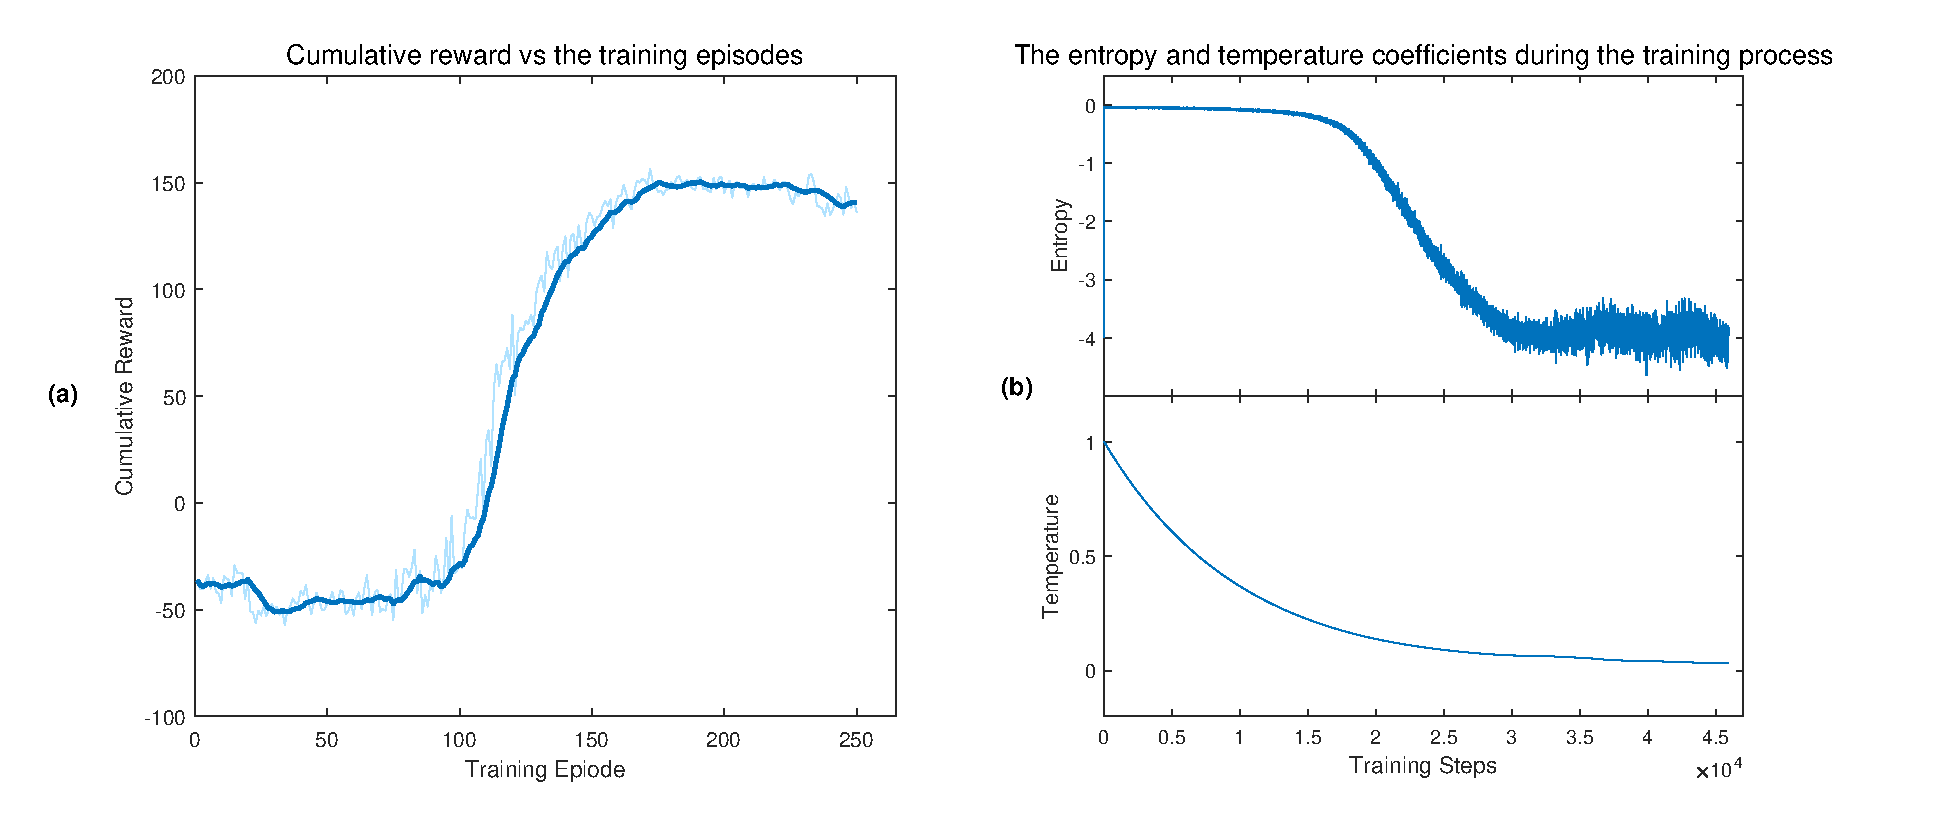
\includegraphics[width=\linewidth]{img/chap5/MBRL_tr.eps}
    \caption{The Training Results of MBRL. (a) Cumulative reward in MBRL vs the training episodes; (b) The variation of entropy and temperature parameters during the training process.}
    \label{fig:MBRL_tr}
\end{figure}

The training progress, along with the entropy and temperature parameters, is visually represented in Figure \ref{fig:MBRL_tr}. The plot illustrates the successful training of the agent using the SAC algorithm. The cumulative reward steadily increased from approximately -45 to 150, indicating the acquisition of the desired behavior by the agent. Additionally, the entropy decreased to around -4 (with the goal being the negative of the number of actions), and the temperature parameter also exhibited a decline from 1 to 0.05. These trends signify that the agent effectively learned the desired behavior during the training phase. Subsequent to the training process, the trained agent was implemented in simulation to evaluate its performance. The results of this implementation are elucidated in Figure \ref{fig:MBRL_val}, providing valuable insights into how well the trained MBRL model performs in executing optimal gaits for the SoftQ. 

Post-training validation in the simulation environment, conducted for a duration of 5 seconds, yielded noteworthy observations. As depicted in the figure, the robot exhibited some velocity along the x-axis. However, it remained virtually stationary at its initial position, effectively patrolling within a confined area. Despite generating speed, the robot failed to manifest any significant forward displacement. This phenomenon is notably characterized by a marked increase in the \ac{COT} during the initial phases of robot motion. This surge in \ac{COT} can be attributed to the imperative need for the robot to surmount inertia and initiate acceleration as it commences motion. Consequently, a substantial input of energy is necessitated. Additionally, heightened frictional forces encountered by mechanical components, such as wheels and joints, during the initial moments of motion contribute to this increased energy expenditure. In addition, the COT is defined as $$COT = \frac{E}{md}$$ where $E$ is the energy consumed to walk, $m$ is the mass of the robot and $d$ represents the distance travelled by the robot.

\begin{figure}[htb]
    \centering
    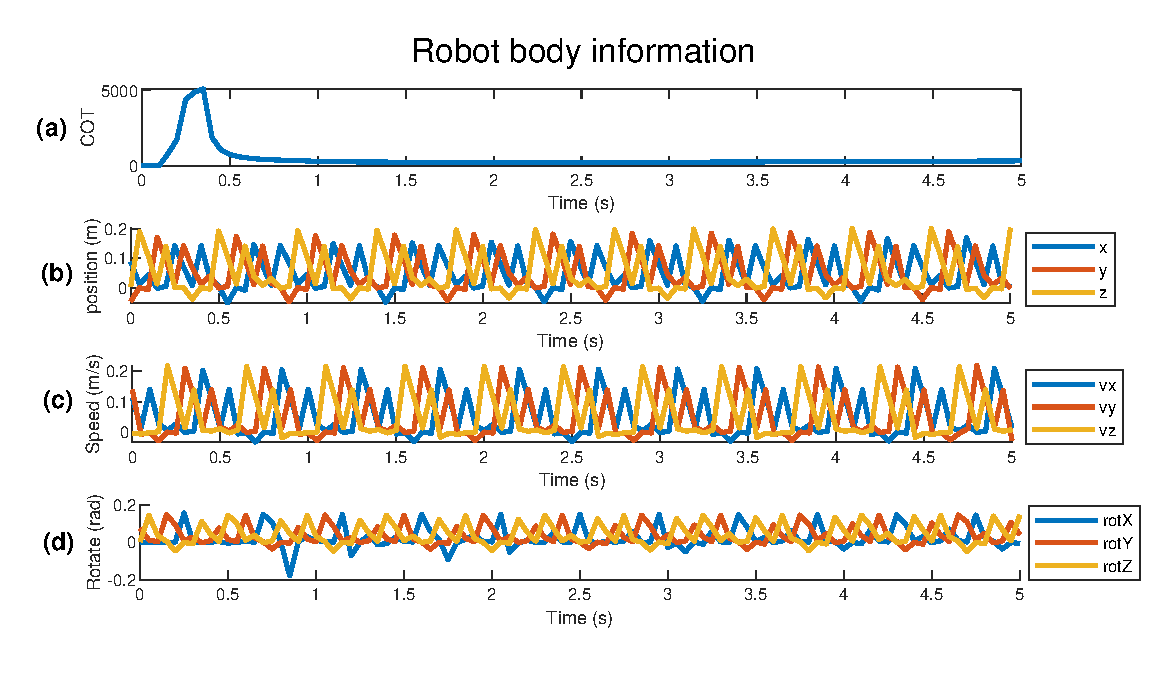
\includegraphics[width=\linewidth]{img/chap5/MBRL_val.eps}
    \caption{The Validation Results of MBRL. (a) COT of the robot while walking; (b) Distance traveled along the $x$, $y$, and $z$ axis; (c) Speed of the robot along the $x$, $y$, and $z$ axis; (d) Orientation of the robot along the $x$, $y$, and $z$ axis.}
    \label{fig:MBRL_val}
\end{figure}

To assess the operational capacity and explore the gait patterns of the soft robot, the same RL configurations were applied to learn optimal gaits under different reference speeds denoted as $v_{ref}$. Throughout the training experiments, an interesting observation emerged: the training performance of the simulated robot was notably influenced by the reference speed $v_{ref}$. When the target velocity was set higher, the learning agent was able to achieve forward motion in fewer training episodes, ultimately converging to an effective policy. Conversely, when $v_{ref}$ was set to a lower value, the agent exhibited a tendency to pitch forward, resulting in episode termination. The training process was initiated with various random seeds, and it was observed that training had a higher failure rate when the agent became trapped in local minima. Consequently, it can be intuitively inferred that mastering the policy for low-speed locomotion posed a more challenging task for the agent.

Given the limitations observed in the direct application of the agent trained through MBRL, a decision was made to further train this agent in a model-free environment to bridge the reality gap effectively. It is noteworthy that adjustments were made to the reward structure, particularly in penalizing instances where all four legs bent in the same direction with a significant angle. The coefficient $\epsilon_4$ governing this penalty was increased from 10 to 100. This modification was introduced due to the possibility that the model-based training might generate actions that are fatal in simulation but less perilous in the real-world scenario.

\subsection{Continue Learning}
To accelerate the training process, a predefined expert behavior, denoted as $A^e = [\textbf{a}_{T_0}^e, ..., \textbf{a}_T^e]$, is established\cite{jiSynthesizingOptimalGait2022}. This predefined behavior offers the robot an initial stable gait. Specifically, during the initial second of each training episode, the RL agent emulates human knowledge by executing the predefined behavior $A^e$. By this means, we resort to the framework of \textit{imitate learning}\cite{koberImitationReinforcementLearning2010}. Data generated from this process is collected and stored in a replay buffer for subsequent learning phases. This approach aligns with the principles of imitation learning, where the RL agent imitates pre-established behaviors as a form of guidance. While it's important to note that this predefined state-action trajectory doesn't guarantee optimality, it serves as a valuable reference for the agent. Emulating these guided elementary movements enables the agent to swiftly implement and adapt its behavior in real-time scenarios, contributing to efficient online implementation. 

To continue training the agent from MBRL, the same RL configurations were applied, with the exception of the penalty adjustment for the four legs bending. The goal for the robot was to learn an optimal gait for higher speed, with $v_{ref}$ set at 0.3 m/s. The reward functions remained the same as defined in Equation \ref{eq:reward}, but the coefficients were adjusted to $[\epsilon_1, \epsilon_2, \epsilon_3, \epsilon_4, \epsilon_5] = [5, −1/v_{ref}, 0.25, 100, 3]$. 

The results of continuous training are visualized in Figure \ref{fig:MFRLvsCT} for comparison with Model-Free Reinforcement Learning (MFRL). Notably, it is observed that the continuous training policy exhibited rapid improvement, reaching convergence at around 200 episodes. However, it's important to note that this policy incurs higher penalties, aligning with the assumption that the MBRL policy may generate riskier actions. Additionally, the MFRL policy converges at approximately 120 episodes, which is slower than the continuous training agent. However, the reward at the beginning of training is higher for MFRL, indicating that the agent in early training may not actively promote forward motion but is associated with fewer high-risk actions. Furthermore, the MFRL approach failed to converge to a walking gait even after 400 episodes, and the MFRL agent did not learn to travel a significant distance. Notably, the MFRL method required about 24 hours of training, while MBRL and continuous training together took approximately 10.5 hours. This substantial reduction in training time, coupled with the ability to achieve effective learning and improved gait control, underscores the efficiency and effectiveness of the continuous training approach compared to the benchmark MFRL method.
\begin{figure}[htb]
    \centering
    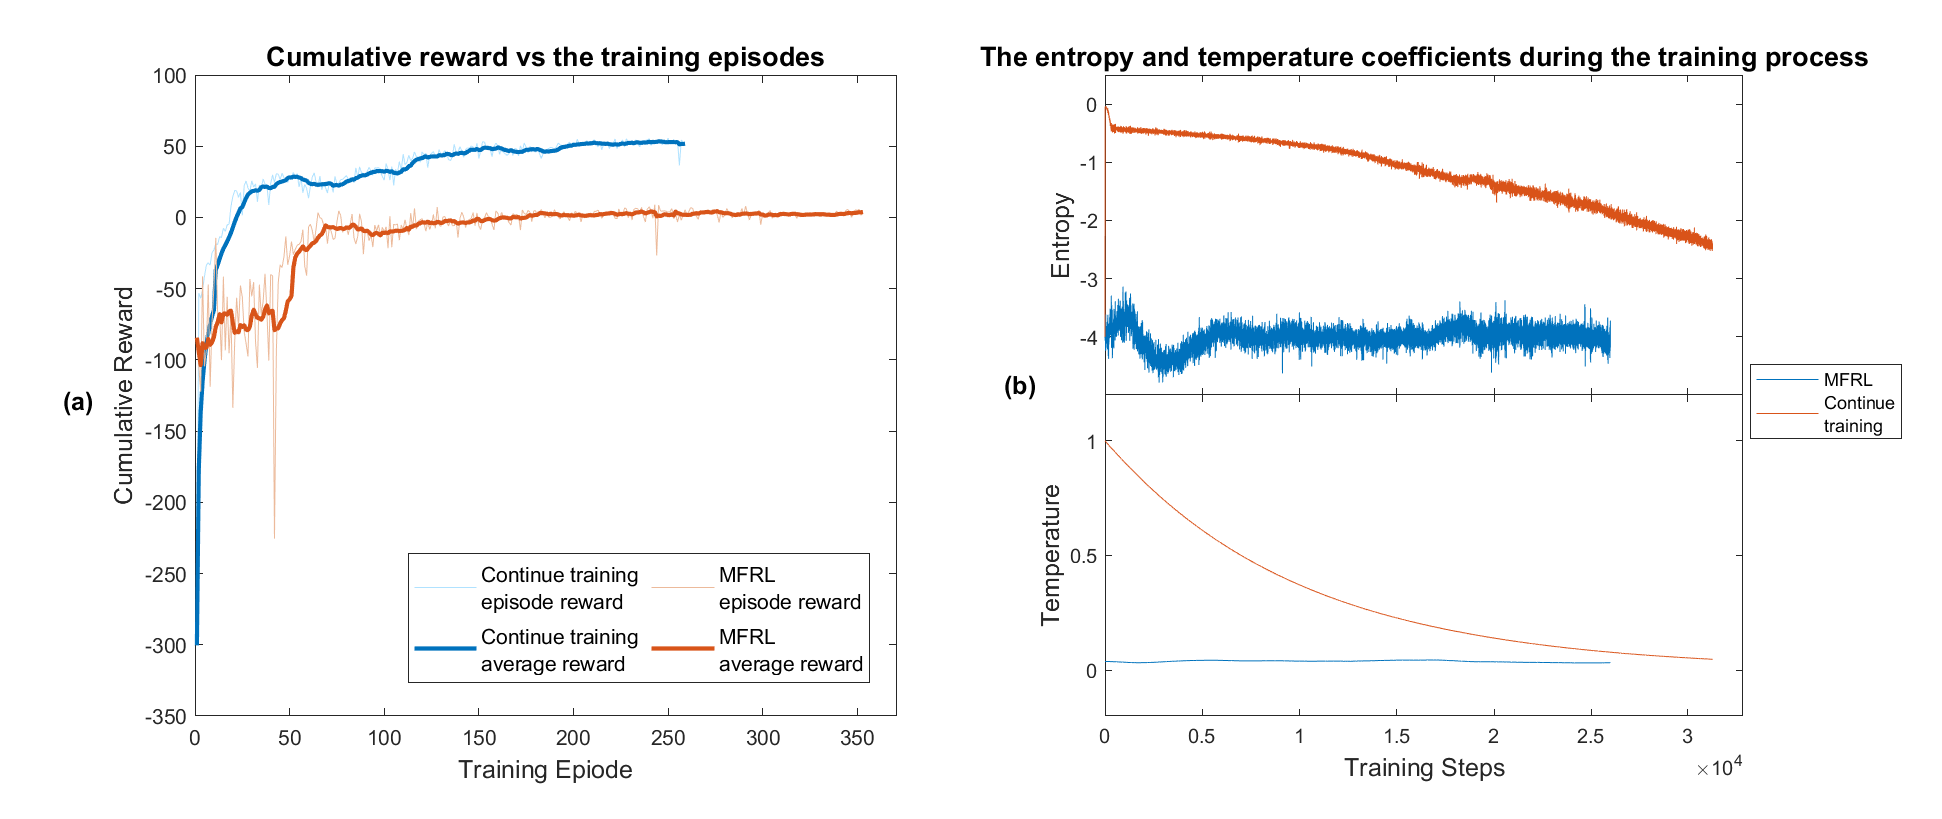
\includegraphics[width=\linewidth]{img/chap5/MFRLvsCT.eps}
    \caption{The Training Results of Continuous Training Compared to MFRL. (a) Cumulative reward in MFRL and continuous training vs the training episodes; (b) The variation of entropy and temperature coefficients during the training process of both MFRL and continuous training.}
    \label{fig:MFRLvsCT}
\end{figure}

The outcomes of validations for continuous training are graphically presented in Figure \ref{fig:CT}, which serves as a overview of continuous training performance. The COT achieved a remarkable low value of approximately 73 J/kg/m, signifying the robot's ability to traverse a certain distance with efficient energy consumption. However, it's worth noting that at the beginning of movement, the COT exhibited a notable increase, reaching approximately 200 J/kg/m. This initial rise in COT can be attributed to several factors, such as static friction, initiate acceleration, and control and actuator-related challenges during the transition from rest to motion. Despite this initial increase in COT, the robot demonstrated its capability to efficiently attain and sustain a speed higher than the predefined benchmark, as attached in Appendix Figure \ref{fig:expert_val}. Over a 5-second validation period, the robot covered a distance of 1.8 meters, achieving an average speed of 0.36 m/s, surpassing the reference speed of 0.3 m/s. These findings highlight the agent's capability to attain and sustain a speed higher than the predefined benchmark. Moreover, the robot demonstrated stability during locomotion, as indicated by the minor fluctuations in velocity along the $x$-axis and minimal deviations in the $y$ and $z$ axes. The orientation plots revealed controlled movement, with the largest rotation measuring approximately 0.055 radians in the initial stages, confirming a stable and well-maintained gait. Collectively, these validation results underscore the practical viability of the continuous training technique in enhancing the robot's performance in real-world scenarios.

\begin{figure}[htb]
    \centering
    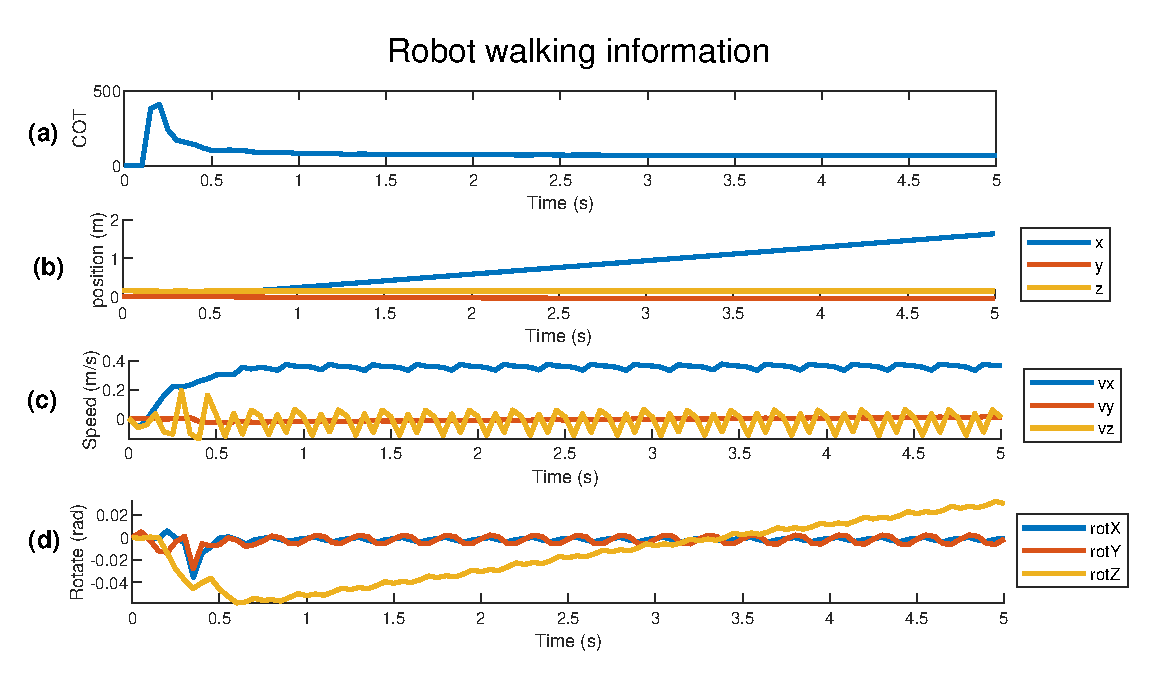
\includegraphics[width=0.9\linewidth]{img/chap5/best_CL.eps}
    \caption{The Validation Results of Continuous Training. (a) COT of the robot while walking; (b) Distance traveled along the $x$, $y$, and $z$ axis; (c) Speed of the robot along the $x$, $y$, and $z$ axis; (d) Orientation of the robot along the $x$, $y$, and $z$ axis.}
    \label{fig:CT}
\end{figure}

Figure \ref{fig:CT_gait} (a) shows the examples of the four foot trajectories, and Figure \ref{fig:CT_gait} (b) with colored areas representing the contact regions demonstrates a typical gait patterns captured from the validation simulation. Synchronized motions were observed between the FR and RL legs, as well as the FL with RR legs, as they are linked as pairs. Notably, the FL and RR leg pairs exhibit a smaller swing area compared to the FR and RL pairs. This difference in swing area may be attributed to corrective actions addressing yaw rotation errors. These yaw rotation errors could potentially be caused by slight uneven mass distribution on the robot, favoring the right side, as indicated by the orientation in the $z$ axis shown in Figure \ref{fig:CT} (d). Additionally, a delay of approximately 0.1 seconds is observed between each diagonal leg pair. The contact time for each leg is around 0.15 seconds, resulting in the formation of a periodic gait pattern. This pattern indicates that the robot successfully learned to coordinate its movements in a rhythmic manner, which is essential for stable and sustained locomotion.

\begin{figure}[htb]
    \centering
    \begin{subfigure}[b]{0.45\textwidth}
    \centering
    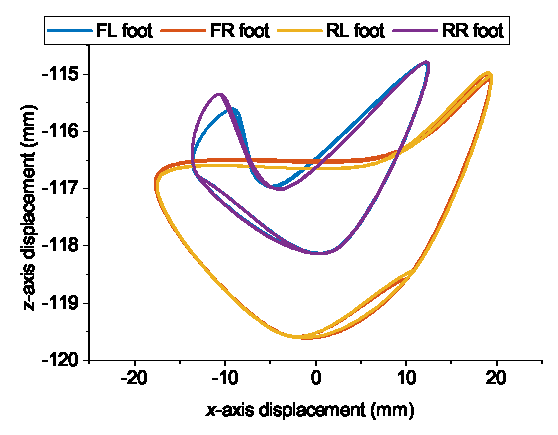
\includegraphics[width=\linewidth]{img/chap5/foot_trace.eps}
    \caption{}
    \end{subfigure}
    \begin{subfigure}[b]{0.45\textwidth}
    \centering
    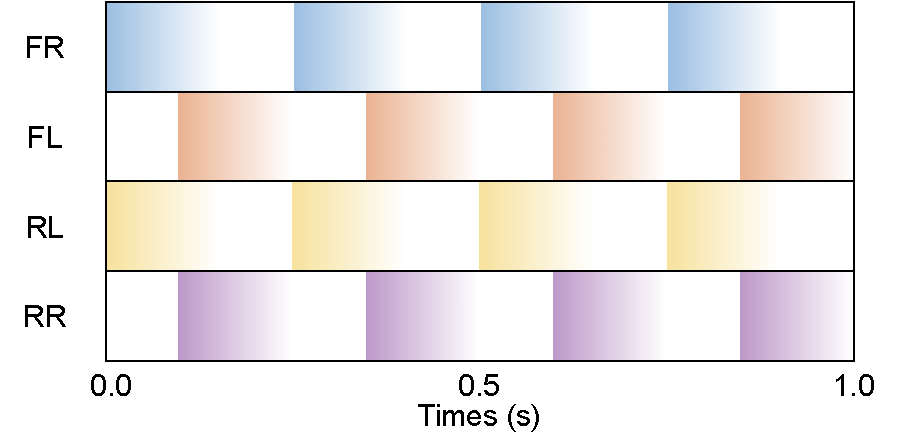
\includegraphics[width=\linewidth]{img/chap5/pattern.pdf}
    \caption{}
    \end{subfigure}
    \caption{The Learned gait patterns. (a) Four foot moving trajectories. (b) Footfall patterns}
    \label{fig:CT_gait}
\end{figure}

Moreover, it's essential to highlight that the observed results go beyond demonstrating successful gait patterns and stability. They also reveal the practical significance of this achievement in terms of direction control within velocity control. As shown in Figure \ref{fig:CT} (d), in the beginning of walking, the robot initially turns to the right but subsequently corrects itself, adjusting its orientation slightly to the left by the end of the gait cycle. This phenomenon was also observed in field tests, as presented in Section \ref{video}. This capability for self-correction and precise direction control enhances the robot's suitability for applications that require controlled and accurate movement, further expanding its utility in real-world scenarios. 

\section{Model-based RL Comparison}
\label{Sec:MBRL}
In order to examine the operational capacity and investigate the gait patterns of the soft robot, we applied the above RL setups to learn the walking motions with different speed references $v_{ref}$, where the training settings are identical in each experiment. During the training experiments, we observe that the training performance of the simulated robot is susceptible to the reference speed $v_{ref}$. With a higher target velocity, the agent is able to walk forward in fewer training episodes with a converged policy. On the other hand, with a smaller $v_{ref}$ as the target, the agent is prone to pitch forward and the episode is terminated. We start the training process with various random seeds, and the training has a higher failure rate with the agent stuck in the local minimal. Hence intuitively, we regard mastering the low-speed locomotion policy as a more difficult task for the agent.

\subsection{Performance Evaluation}
In the performance evaluation of the trained agent, it is important to consider several critical metrics. These metrics serve as crucial indicators of proficiency of the agent, referred to as the controller. Here, these metrics are expounded again avoiding excessive details:
\begin{itemize}
    \item Stability : This metric combines information about the time duration of the gait, rotational motion, and vertical displacement to assess the stability of the gait. It provides valuable insights into the agent's ability to maintain stability during operation. 
    \item Resultant walking speed (m/s): This metric involves assessing the agent's walking speed, particularly by calculating the average speed achieved during validation. It offers a straightforward measure of the agent's mobility and effectiveness in movement.
    \item Cost-of-Transport (J/kg/m):  The COT metric evaluates the energy efficiency of the agent. It quantifies the amount of energy expended by the agent, normalized by its weight and the distance traveled. This metric is crucial for understanding the agent's energy consumption patterns.
    \item Learning efficiency:  Learning efficiency gauges how quickly the agent converges to an optimal or satisfactory performance level. It is quantified by measuring the training time required for the agent to reach convergence and the reward reach a significant level. This metric provides insights into the agent's adaptability and learning capabilities.
\end{itemize}

\subsection{Compare with MFRL}
This section will delve into the performance comparison between the MBRL with continuous training and MFRL based metrics outlined earlier. To ensure a robust evaluation, three identical training sessions were conducted for each reference velocity $v_{ref}$, which took values of 0.2 m/s, 0.3 m/s, and 0.5 m/s. Training was stopped upon the convergence of each policy to a significant reward level. Following the training phase, each trained agent was implemented and evaluated through simulation of 5s. The results of these evaluations are visually represented in Figure \ref{fig:box}. It is evident from the figure that MBRL with continuous training consistently outperforms MFRL. This conclusion is drawn based on the observation that the mean values of key performance metrics, including stability, resultant walking speed, COT, and training time, are consistently higher for MBRL with continuous training compared to MFRL. 

Specifically, in terms of stability, MBRL with continuous training achieved a mean stability level of approximately 0.62, significantly surpassing MFRL, which achieved a mean stability of approximately 0.1. Notably, the level of stability achieved by MBRL with continuous training closely approximated that of the predefined expert gait, indicating its capability to generate highly stable locomotion. 
\begin{figure}[htb]
    \centering
    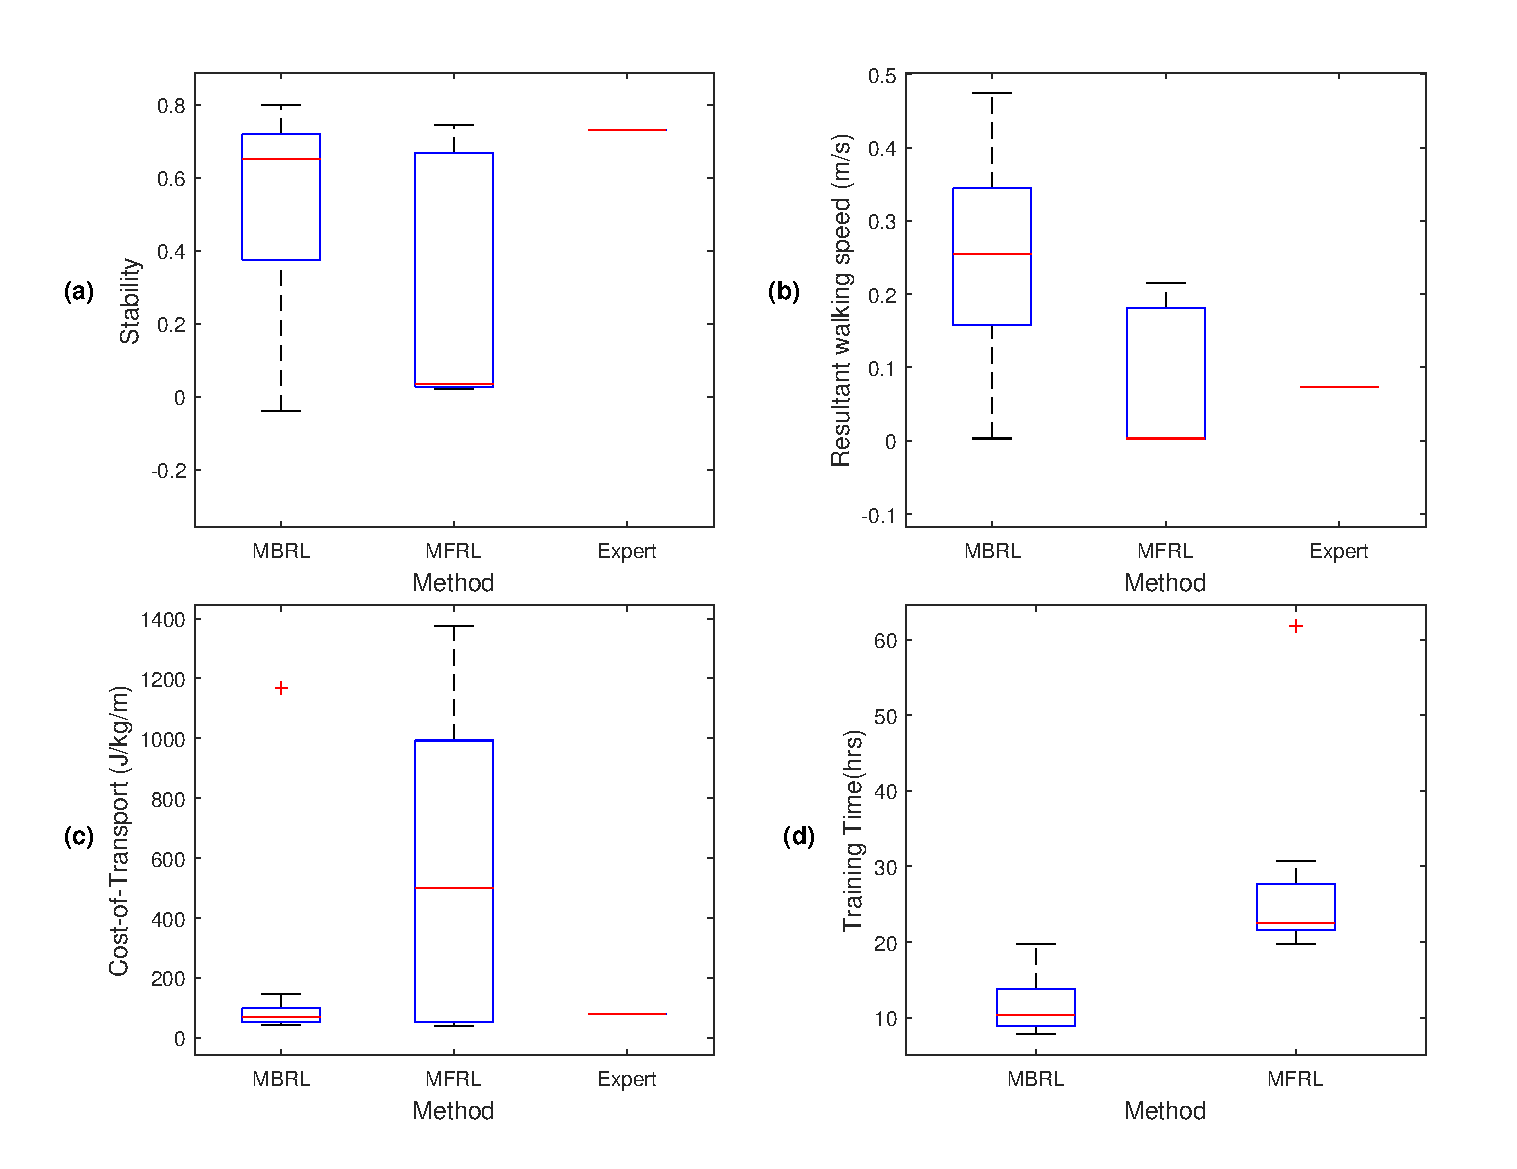
\includegraphics[width=\linewidth]{img/chap5/box_results.eps}
    \caption{The Box Plot of MBRL with Continuous Training compared to MFRL. (a) Box plot of stability by method; (b) Box plot of resultant walking speed by method ; (c) Box plot of COT by method; (d) Box plot of simulation time by method.}
    \label{fig:box}
\end{figure}

Regarding resultant walking speed, it was noted that MBRL with continuous training exhibited a higher mean walking speed. However, it also displayed a larger variance, partly due to variations in reference walking speeds ($v_{ref}$).Despite the variance, the mean walking speed achieved by MBRL with continuous training was significantly greater than that of MFRL. It's worth noting that MBRL, in its pursuit of efficient locomotion, tended to focus on walking further, resulting in a mean speed that was significantly higher than the expert gait's speed, even though it initially learned from the expert gait. In contrast, MFRL faced challenges in learning extended walking within 400 training episodes, which is reflected in the mean speed approaching zero. It primarily struggled to adapt and achieve higher speeds or longer distances. This disparity in performance between MBRL with continuous training and MFRL underscores the advantages of the former approach in facilitating both stable and efficient locomotion, even surpassing the performance of the expert gait. 

Furthermore, the analysis revealed that MBRL with continuous training achieved an efficient COT level, similar to that of the predefined expert gait, indicating economical energy consumption during locomotion. In contrast, MFRL agents exhibited significantly higher COT values. This difference primarily stemmed from the fact that only a limited number of MFRL agents succeeded in overcoming the initial resistance associated with initiating longer-distance walking. 

Lastly, it was observed that MBRL with continuous training demonstrated superior training efficiency, aligning with the primary objective of this thesis. It exhibited a greater capacity to learn efficient locomotion, particularly for longer distances. Additionally, considering that a smaller fraction of MFRL agents achieved extended walking within 400 episodes, the actual simulation time required for MFRL to achieve comparable results would likely exceed what is presented in Figure \ref{fig:box}(d).

In summary, the findings emphasized the consistent advantages of employing MBRL with continuous training over MFRL in terms of stability, walking speed, energy efficiency, and training effectiveness. Furthermore, MBRL with continuous training not only outperforms MFRL but also attains performance levels similar to those of the predefined expert gait, showcasing its potential for real-world applications where stable and efficient locomotion is of paramount importance.

\subsection{ANCOVA Tests}
However, it is essential to acknowledge that reference walking speed ($v_{ref}$) represents a covariate in this comparative analysis. To ensure a rigorous assessment that accounts for the potential influence of this covariate, an \ac{ANCOVA} was conducted to compare MBRL with continue learning and MFRL. This statistical analysis enabled us to compare these two RL approaches while effectively controlling for the covariate $v_{ref}$. This analysis primarily focused on the following dependent variables, as previously defined in Section \ref{Sec:test_def}: stability, resultant walking speed, COT and learning efficiency. This ANCOVA analysis provides a robust framework for evaluating the relative performance of the two RL approaches, while considering the potential impact of reference walking speed ($v_{ref}$). The results of this analysis offer deeper insights into the effectiveness of each method in achieving stable and efficient gait control for our soft robot. The details of ANCOVA is discussed in \ref{Sec:ANCOVA}.

The hypothesis holds that MBRL with continuous training is significantly more effective and efficient in achieving stable and efficient gait control for our soft robot SoftQ compared to MFRL, across various reference velocities ($v_{ref}$).

\subsubsection*{Stability}
The ANCOVA analysis revealed both the method of RL (MBRL or MFRL) and the covariate $v_{ref}$ have a statistically significant effect on walking stability. The F-value of 5.9902 and the p-value of 0.0307 in the effect of method indicate that the method of RL significantly influences walking stability. Given that the p-value is less than 0.05, this effect is statistically significant, suggesting that one of these methods is likely better than the other in terms of enhancing walking stability. $v_{ref}$ serves as a covariate in this study, and it too shows a statistically significant F-value of 4.3583 and a p-value of 0.0378. This implies that $v_{ref}$ independently impacts walking stability, and its effect is statistically significant. The interaction between the method and $v_{ref}$ is also significant, with an F-value of 5.4802 and a p-value of 0.0204. This suggests that the effect of the learning method on walking stability is not consistent across all levels of $v_{ref}$. In other words, the optimal choice between MBRL and MFRL may depend on the specific value of $v_{ref}$. This suggests that the  RL approaches has a significant positive impact on the stability of walking.

\begin{table}[H]
    \centering
    \begin{tabular}{c|ccccc} 
         Source&  DoF&  Sum Sq&  Mean Sq&  F& Prob>F\\ \hline
         $v_{ref}$&  2&  0.4734&  0.2367&  4.3583& 0.0378\\ 
         Method&  1&  0.3254&  0.3254&  5.9902& 0.0307\\ 
         $v_{ref}\cdot$Method&  2&  0.5953&  0.2977&  5.4802& 0.0204\\ 
         Error&  12&  0.6518&  0.0543&  & \\ 
    \end{tabular}
    \caption{ANCOVA test of stability metrics.}
    \label{tab:ANCOVA_sta}
\end{table}

\subsubsection*{Resultant walking speed}
The ANCOVA analysis concluded that the method of RL significantly impacts resultant walking speed, while $v_{ref}$ does not. The DoF for $v_{ref}$ is 2, and it has a Sum of Squares (Sum Sq) of 0.0056, yielding a Mean Square (Mean Sq) of 0.0028. The F-value is a low 0.2133, and the p-value is notably high at 0.8109. These metrics strongly suggest that $v_{ref}$ does not have a statistically significant impact on the resultant walking speed in this case. The Method has a DoF of 1 with a Sum Sq of 0.1390, resulting in a Mean Sq of 0.1390. The F-value is considerably high at 10.6660, and the p-value is 0.0068, well below the 0.05 threshold. These values point to a statistically significant influence of the RL method on resultant walking speed. This implies that either MBRL or MFRL has a substantial impact on walking speed, warranting further investigation to determine the most effective approach. The interaction term shows a DoF of 2, a Sum Sq of 0.0991, and a Mean Sq of approximately 0.0496. With an F-value of 3.8011 and a p-value of 0.0526, the interaction term is borderline significant. This indicates that the effect of the RL method on resultant walking speed may vary depending on $v_{ref}$, although the evidence is not strong enough to make this conclusion definitively.
\begin{table}[H]
    \centering
    \begin{tabular}{c|ccccc} 
         Source&  DoF&  Sum Sq&  Mean Sq&  F& Prob>F\\ \hline
         $v_{ref}$&  2&  0.0056&  0.0028&  0.2133& 0.8109\\ 
         Method&  1&  0.1390&  0.1390&  10.6660& 0.0068\\ 
         $v_{ref}\cdot$Method&  2&  0.0991&  0.0496&  3.8011& 0.0526\\ 
         Error&  12&  0.1564&  0.0130&  & \\ 
    \end{tabular}
    \caption{ANCOVA test of resultant walking speed.}
    \label{tab:ANCOVA_v}
\end{table}

\subsubsection{Cost-of-Transport}
The data indicates that the choice of RL method (MBRL or MFRL) has a statistically significant impact on COT. On the other hand, the influence of $v_{ref}$ is borderline significant, and the interaction term between $v_{ref}$ and method of RL is not statistically significant. In effect of $v_{ref}$, the F-value stands at 3.7479 with a p-value of 0.0544. While the F-value suggests a reasonable effect, the p-value marginally exceeds the typical 0.05 significance threshold, making the influence of $v_{ref}$ on COT statistically borderline. In effect of RL method, the F-value is 5.5947 with a p-value of 0.0357. Given the p-value is less than 0.05, the influence of the chosen RL method on COT is statistically significant. In the effect of interaction term ($v_{ref}\cdot$Method), the F-value is 2.9587, and the p-value is 0.0902. Although the F-value suggests some degree of effect, the p-value is greater than 0.05, suggesting that the interaction effect is not statistically significant. Therefore, while the RL method appears to be a crucial factor affecting COT, the role of $v_{ref}$ and its interaction with the method may require additional research to be conclusively understood.
\begin{table}[H]
    \centering
    \begin{tabular}{c|ccccc} 
         Source&  DoF&  Sum Sq&  Mean Sq&  F& Prob>F\\ \hline
         $v_{ref}$&  2&  \num{9.5553e5}&  \num{4.7776e5}&  3.7479& 0.0544\\ 
         Method&  1&  \num{7.1318e5}&  \num{7.1318e5}&  5.5947& 0.0357\\ 
         $v_{ref}\cdot$Method&  2&  \num{7.5432e5}&  \num{3.7716e5}&  2.9587& 0.0902\\ 
         Error&  12&  \num{1.5297e6}&  \num{1.747e5}&  & \\ 
    \end{tabular}
    \caption{ANCOVA test of COT.}
    \label{tab:ANCOVA_COT}
\end{table}

\subsubsection{Learning efficiency}
The ANCOVA analysis underscores the statistical significance of the RL method in influencing learning efficiency. The $v_{ref}$ term as a covariate,  is characterized by a Degrees of Freedom (DoF) of 2, Sum of Squares (Sum Sq) of 208.0905, and Mean Square (Mean Sq) of 104.0452. The F-value is 1.2107 and the p-value is 0.3319. Given the p-value is well above the common 0.05 significance threshold, $v_{ref}$ does not appear to have a statistically significant impact on learning efficiency. The Method term has a DoF of 1, a Sum Sq of \num{1.1997e3}, and a Mean Sq of \num{1.1997e3}. The F-value is remarkably high at 13.9597, and the p-value is notably low at 0.0028. These values confirm that the Method is statistically significant in affecting learning efficiency, suggesting a noteworthy influence of the chosen RL approach. The interaction term has a DoF of 2, a Sum Sq of 265.9588, and a Mean Sq of 132.9794. The F-value is 1.5473, and the p-value is 0.2524. These numbers indicate that the interaction term does not meet the threshold for statistical significance, which implies that the effect of the RL method on learning efficiency is generally consistent across different $v_{ref}$ levels. 
 
\begin{table}[H]
    \centering
    \begin{tabular}{c|ccccc} 
         Source&  DoF&  Sum Sq&  Mean Sq&  F& Prob>F\\ \hline
         $v_{ref}$&  2&  208.0905&  104.0452&  1.2107& 0.3319\\ 
         Method&  1&  \num{1.1997e3}&  \num{1.1997e3}&  13.9597& 0.0028\\ 
         $v_{ref}\cdot$Method&  2&  265.9588&  132.9794&  1.5473& 0.2524\\ 
         Error&  12&  \num{1.0313e3}&  85.9405&  & \\ 
    \end{tabular}
    \caption{ANCOVA test of learning efficiency.}
    \label{tab:ANCOVA_time}
\end{table}

\section{Field Test}
The culmination of the MBRL and continuous training efforts is the deployment of the trained controller onto the physical SoftQ robot. This section presents the results of the field tests, providing insights into the controller's transferability, generalization capabilities, and its performance in real-world scenarios.

The primary objective of the field tests is to evaluate the extent to which the controller's learned policy can be transferred from the simulated environment to the physical robot. To facilitate these tests, two room dividers are placed at the front and side of the robot to form the test field and reflect the light signals from the ToF sensors as well as the localization references for the robot. The task assigned to the robot is to walk from its initial position towards the front divider and stop at a distance of 0.3 m to the front divider, the total walking distance is approximately 1.5 m. 

The directly learned walking gait for $v_{ref} = 0.3m/s$ was tested on the real robot of SoftQ. Figure \ref{fig:real_test} provides a photographic stills of the field test at various time stamps. It begins with the robot's initial starting point (a) and progresses through its forward movement with the trained control policy at different time intervals (b - e). Finally, the robot successfully completes the 1.5-meter walk in 10 seconds and stands at the designated endpoint (f). These field tests demonstrate the exceptional transferability and adaptability of the controller, showcasing its ability to seamlessly apply learned behaviors in real-world scenarios. The successful execution of the task underscores the practical viability of our approach, emphasizing the potential for real-world applications where precise locomotion and control are essential.

\begin{figure}[htb]
    \centering
    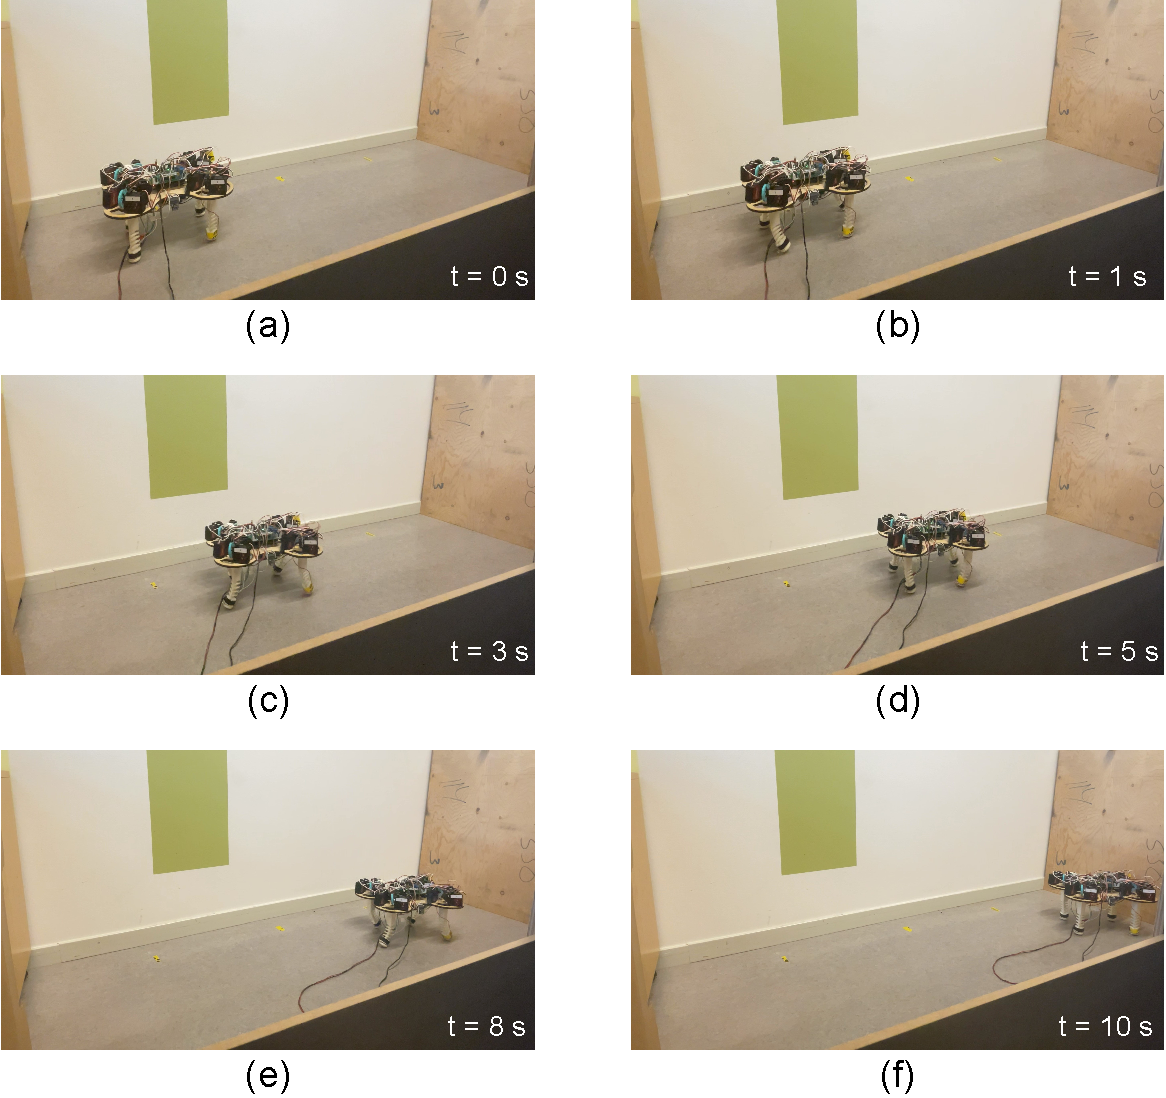
\includegraphics[width=0.9\linewidth]{img/chap5/real_test.pdf}
    \caption{Snapshots at Different Time Stamps of the Field Test of SoftQ Walking. (a) The initial start point of the robot SoftQ. (b - e) The robot walked forward with the trained control policy at different time while walking. (f) , the robot finished walking at the designated endpoint.}
    \label{fig:real_test}
\end{figure}

Figure \ref{fig:real_v} shows the recorded speed change in the three directions of the robot center. The speed in the forward direction starts around 0.2 m/s, represented by the filtered curve of the forward speeds. This speed then decreases to around -0.1 m/s before gradually increasing to approximately 0.4 m/s. Subsequently, the speed fluctuates between 0 m/s and 0.3 m/s until it reaches the endpoint. The resultant walking speed, calculated based on the total distance traveled, averages around 0.15 m/s. It's noteworthy that this achieved speed is somewhat lower than the target speed of 0.3 m/s in the simulation. This discrepancy can be attributed to the reality gap caused by inaccuracies in the model's actuators, sensors, and foot-ground contact dynamics. In the lateral directions ($y$ and $z$), observable speed perturbations are present, particularly in the $z$ axis. These fluctuations indicate the robot's rapid vertical motion, ranging from -0.6 m/s to 0.6 m/s. The $y$-axis velocities range from -0.4 m/s to 0.3 m/s, which may be attributed to self-corrections and lateral movements during walking. 

\begin{figure}[htb]
    \centering
    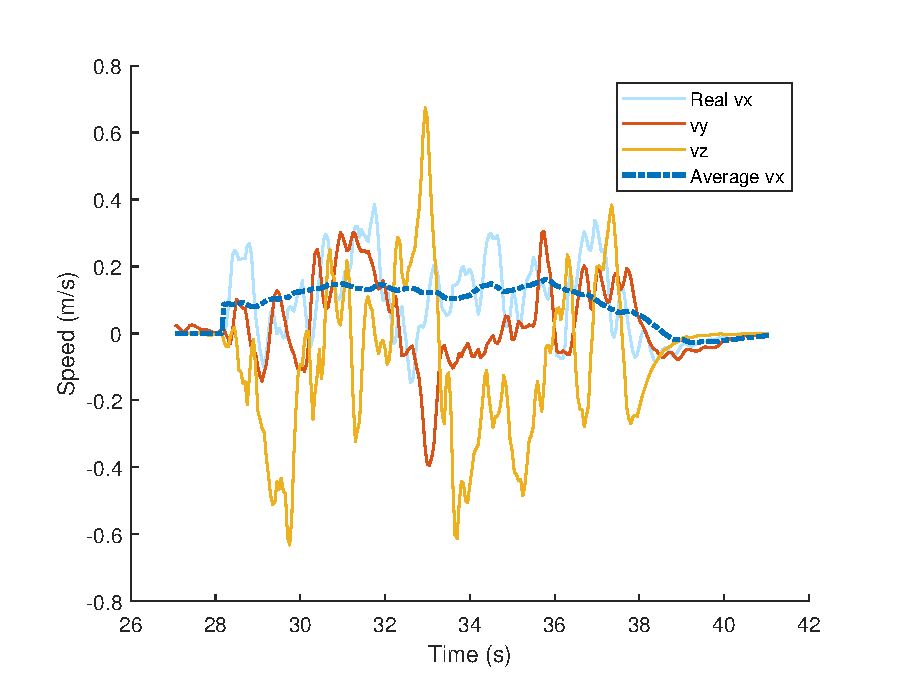
\includegraphics[width=0.9\linewidth]{img/chap5/real_v.eps}
    \caption{The field test results of measurement of velocity at $x$, $y$ and $z$ axis.}
    \label{fig:real_v}
\end{figure}

These results underscore the exceptional transferability and generalization capabilities of the trained controller, highlighting its ability to adapt learned behaviors to real-world settings despite disparities between the simulation and the physical environment. The field tests further emphasize the controller's impressive locomotion performance across various terrains and conditions, providing evidence of its adaptability and robustness in practical scenarios. The outstanding performance observed in the field tests holds significant implications for the power of this methodology enhanced by MBRL. The robot prototype successfully completes the preliminary walking test under real-time execution by utilizing the SAC trained agents.